%------------------------------------------------------------------------------------------------------------------------
\chapter{現行ピクセルモジュールの電荷較正}
\label{sec:chap3}
%------------------------------------------------------------------------------------------------------------------------

本章では、ASICから得られるToT(Time over Threshold)を荷電粒子がシリコンセンサーに落とす電荷に較正する方法について説明する。

%------------------------------------------------------------------------------------------------------------------------
\section{アナログ回路}
\label{sec:analog}
%------------------------------------------------------------------------------------------------------------------------


%------------------------------------------------------------------------------------------------------------------------
\section{チューニング}
\label{sec:tuning}
%------------------------------------------------------------------------------------------------------------------------
各ピクセルにおけるThresholdと、ある基準電荷量の信号に対するToTを任意の値に調整するためにASICのチューニングを行う。Thresholdおよび任意の値に対するToTの目標値をそれぞれ\tref{tab:thresholdtuning}、\tref{tab:tottuning}に示す。

\begin{table}[tbp]
  \begin{center}
    \caption[各LayerにおけるThresholdの値]{各LayerにおけるThresholdの値。}
    \label{tab:thresholdtuning}
    \begin{tabular}{|l||r|r|r|r|}
    \hline
      Layer名  & 2015年($4\ \si{fb^{-1}}$) & 2016年($39\ \si{fb^{-1}}$) & 2017年($50\ \si{fb^{-1}}$) & 2018年($63\ \si{fb^{-1}}$) \\
    \bhline{1.5pt}
      IBL & $2500\ (\mathrm{ToT}>2)$ & $2500\ (\mathrm{ToT}>2)$ & $2500\ (\mathrm{ToT}>2)$ & $2000\ (\mathrm{ToT}>2)$ \\
    \hline
      B-Layer (中心付近) & $3500\ (\mathrm{ToT}>3)$ & $3500\ (\mathrm{ToT}>3)$ & $5000\ (\mathrm{ToT}>5)$ & $4300\ (\mathrm{ToT}>3)$ \\
    \hline
      B-Layer (前方付近) & $3500\ (\mathrm{ToT}>3)$ & $3500\ (\mathrm{ToT}>3)$ & $5000\ (\mathrm{ToT}>5)$ & $5000\ (\mathrm{ToT}>5)$ \\
    \hline
      Layer1 & $3500\ (\mathrm{ToT}>3)$ & $3500\ (\mathrm{ToT}>5)$ & $3500\ (\mathrm{ToT}>5)$ & $3500\ (\mathrm{ToT}>5)$ \\
    \hline
      Layer2 & $3500\ (\mathrm{ToT}>3)$ & $3500\ (\mathrm{ToT}>5)$ & $3500\ (\mathrm{ToT}>5)$ & $3500\ (\mathrm{ToT}>5)$ \\
    \hline
      Disk & $3500\ (\mathrm{ToT}>3)$ & $3500\ (\mathrm{ToT}>5)$ & $4500\ (\mathrm{ToT}>8)$ & $3500\ (\mathrm{ToT}>5)$ \\
    \hline
    \end{tabular}
  \end{center}
\end{table}

\begin{table}[tbp]
  \begin{center}
    \caption[各LayerにおけるToTのチューニングの値]{各LayerにおけるToTのチューニングの値。}
    \label{tab:tottuning}
    \begin{tabular}{|l||r|r|r|r|}
    \hline
      Layer名  & 2015年($4\ \si{fb^{-1}}$) & 2016年($39\ \si{fb^{-1}}$) & 2017年($50\ \si{fb^{-1}}$) & 2018年($63\ \si{fb^{-1}}$) \\
    \bhline{1.5pt}
      IBL & $10 \mathrm{ToT} (16\ \si{ke})$ & $8 \mathrm{ToT} (16\ \si{ke})$ & $8 \mathrm{ToT} (16\ \si{ke})$ & $10 \mathrm{ToT} (16\ \si{ke})$ \\
    \hline
      B-Layer & $30 \mathrm{ToT} (20\ \si{ke})$ & $30 \mathrm{ToT} (20\ \si{ke})$ & $30 \mathrm{ToT} (20\ \si{ke})$ & $30 \mathrm{ToT} (20\ \si{ke})$ \\
    \hline
      Layer1 & $30 \mathrm{ToT} (20\ \si{ke})$ & $30 \mathrm{ToT} (20\ \si{ke})$ & $30 \mathrm{ToT} (20\ \si{ke})$ & $30 \mathrm{ToT} (20\ \si{ke})$ \\
    \hline
      Layer2 & $30 \mathrm{ToT} (20\ \si{ke})$ & $30 \mathrm{ToT} (20\ \si{ke})$ & $30 \mathrm{ToT} (20\ \si{ke})$ & $30 \mathrm{ToT} (20\ \si{ke})$ \\
    \hline
      Disk & $30 \mathrm{ToT} (20\ \si{ke})$ & $30 \mathrm{ToT} (20\ \si{ke})$ & $30 \mathrm{ToT} (20\ \si{ke})$ & $30 \mathrm{ToT} (20\ \si{ke})$ \\
    \hline
    \end{tabular}
  \end{center}
\end{table}

チューニングには、あるASICにおける全ピクセルのTresholdと任意の値に対するToTを調整するためのglobalチューニングと各ピクセルごとの値を目標値に近づけるlocalチューニングがある。はじめに、globalチューニングを行い、全ピクセルのThresholdまたはToTを大まかに目標値に合わせる。この段階では、全ピクセルから得られる分布の分散は大きいため、localチューニングを行い各ピクセルが返す値を目標値にさらに近づける。
%ToTの値はThresholdに依存するため、Thresholdのチューニングの前後においてToTが変わってしまう。また、同様にToTチューニングの後はThreshold値が変化してしまう。この影響は、チューニングを繰り返すことで小さくなり、

チューニングの後、ThresholdスキャンやToTスキャンを行い各ピクセルにおける値を測定する。ThresholdおよびToTスキャンの方法を以下に述べる。

%------------------------------------------------------------------------------------------------------------------------
\subsubsection{Thresholdスキャン}
\label{sec:thresholdscan}
%------------------------------------------------------------------------------------------------------------------------
Thresholdスキャンでは、各ピクセルに試験電荷を入射しThresholdとノイズを測定する。試験電荷を増加させつつ検出効率を測定し、\fref{fig:threshold}に示す様な分布を作成する。この分布はS字を描くため、\textbf{Sカーブ}と呼ばれている。\fref{fig:threshold}中の青線はSカーブふのフィッティングであり、\eref{eq:gosakannsuu}のような誤差関数を用いて定義される。
\begin{equation}
  \label{eq:gosakannsuu}
  f(x)=0.5\times\left[ 2-\mathrm{erfc}\left( \frac{x-Q_\mathrm{threshold}}{\sigma \times \sqrt{2}} \right)  \right] \times p
\end{equation}
Sカーブにおいて、検出効率が$50\%$となる試験電荷の値をThresholdと定義し、検出効率が$83.5\%$と$16.5\%$となる試験電荷の幅をノイズと定義する。

\begin{figure}[tbp]
  \centering
  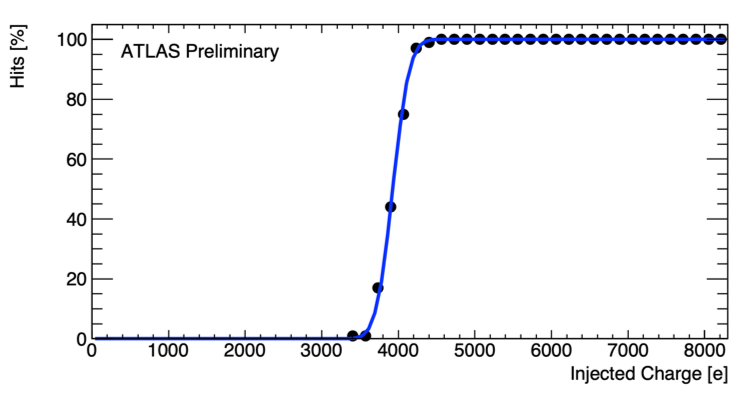
\includegraphics[height=5cm,keepaspectratio]{threshold.png}
  \caption[検出効率と試験電荷の関係]{検出効率と試験電荷の関係。}
  \label{fig:threshold}
\end{figure}


%------------------------------------------------------------------------------------------------------------------------
\subsubsection{ToTスキャン}
\label{sec:totscan}
%------------------------------------------------------------------------------------------------------------------------
ToTスキャンでは、一定の試験電荷を各ピクセルに100回入射させ、その試験電荷に対するToTの値の測定を行う。各ピクセルから得られるToTの値はデジタル値であるため整数値であるが、100回のスキャンの平均値をある試験電荷に対するToTとするため、この値は小数値を取り得る。


%------------------------------------------------------------------------------------------------------------------------
\section{電荷較正}
\label{sec:calibration}
%------------------------------------------------------------------------------------------------------------------------


%------------------------------------------------------------------------------------------------------------------------
\section{電荷較正における問題点}
\label{sec:probrem}
%------------------------------------------------------------------------------------------------------------------------



\newpage
